% Agentic RAG với LangGraph 0
\begin{frame}{Agentic RAG với LangGraph}

\begin{figure}[H]
\centering
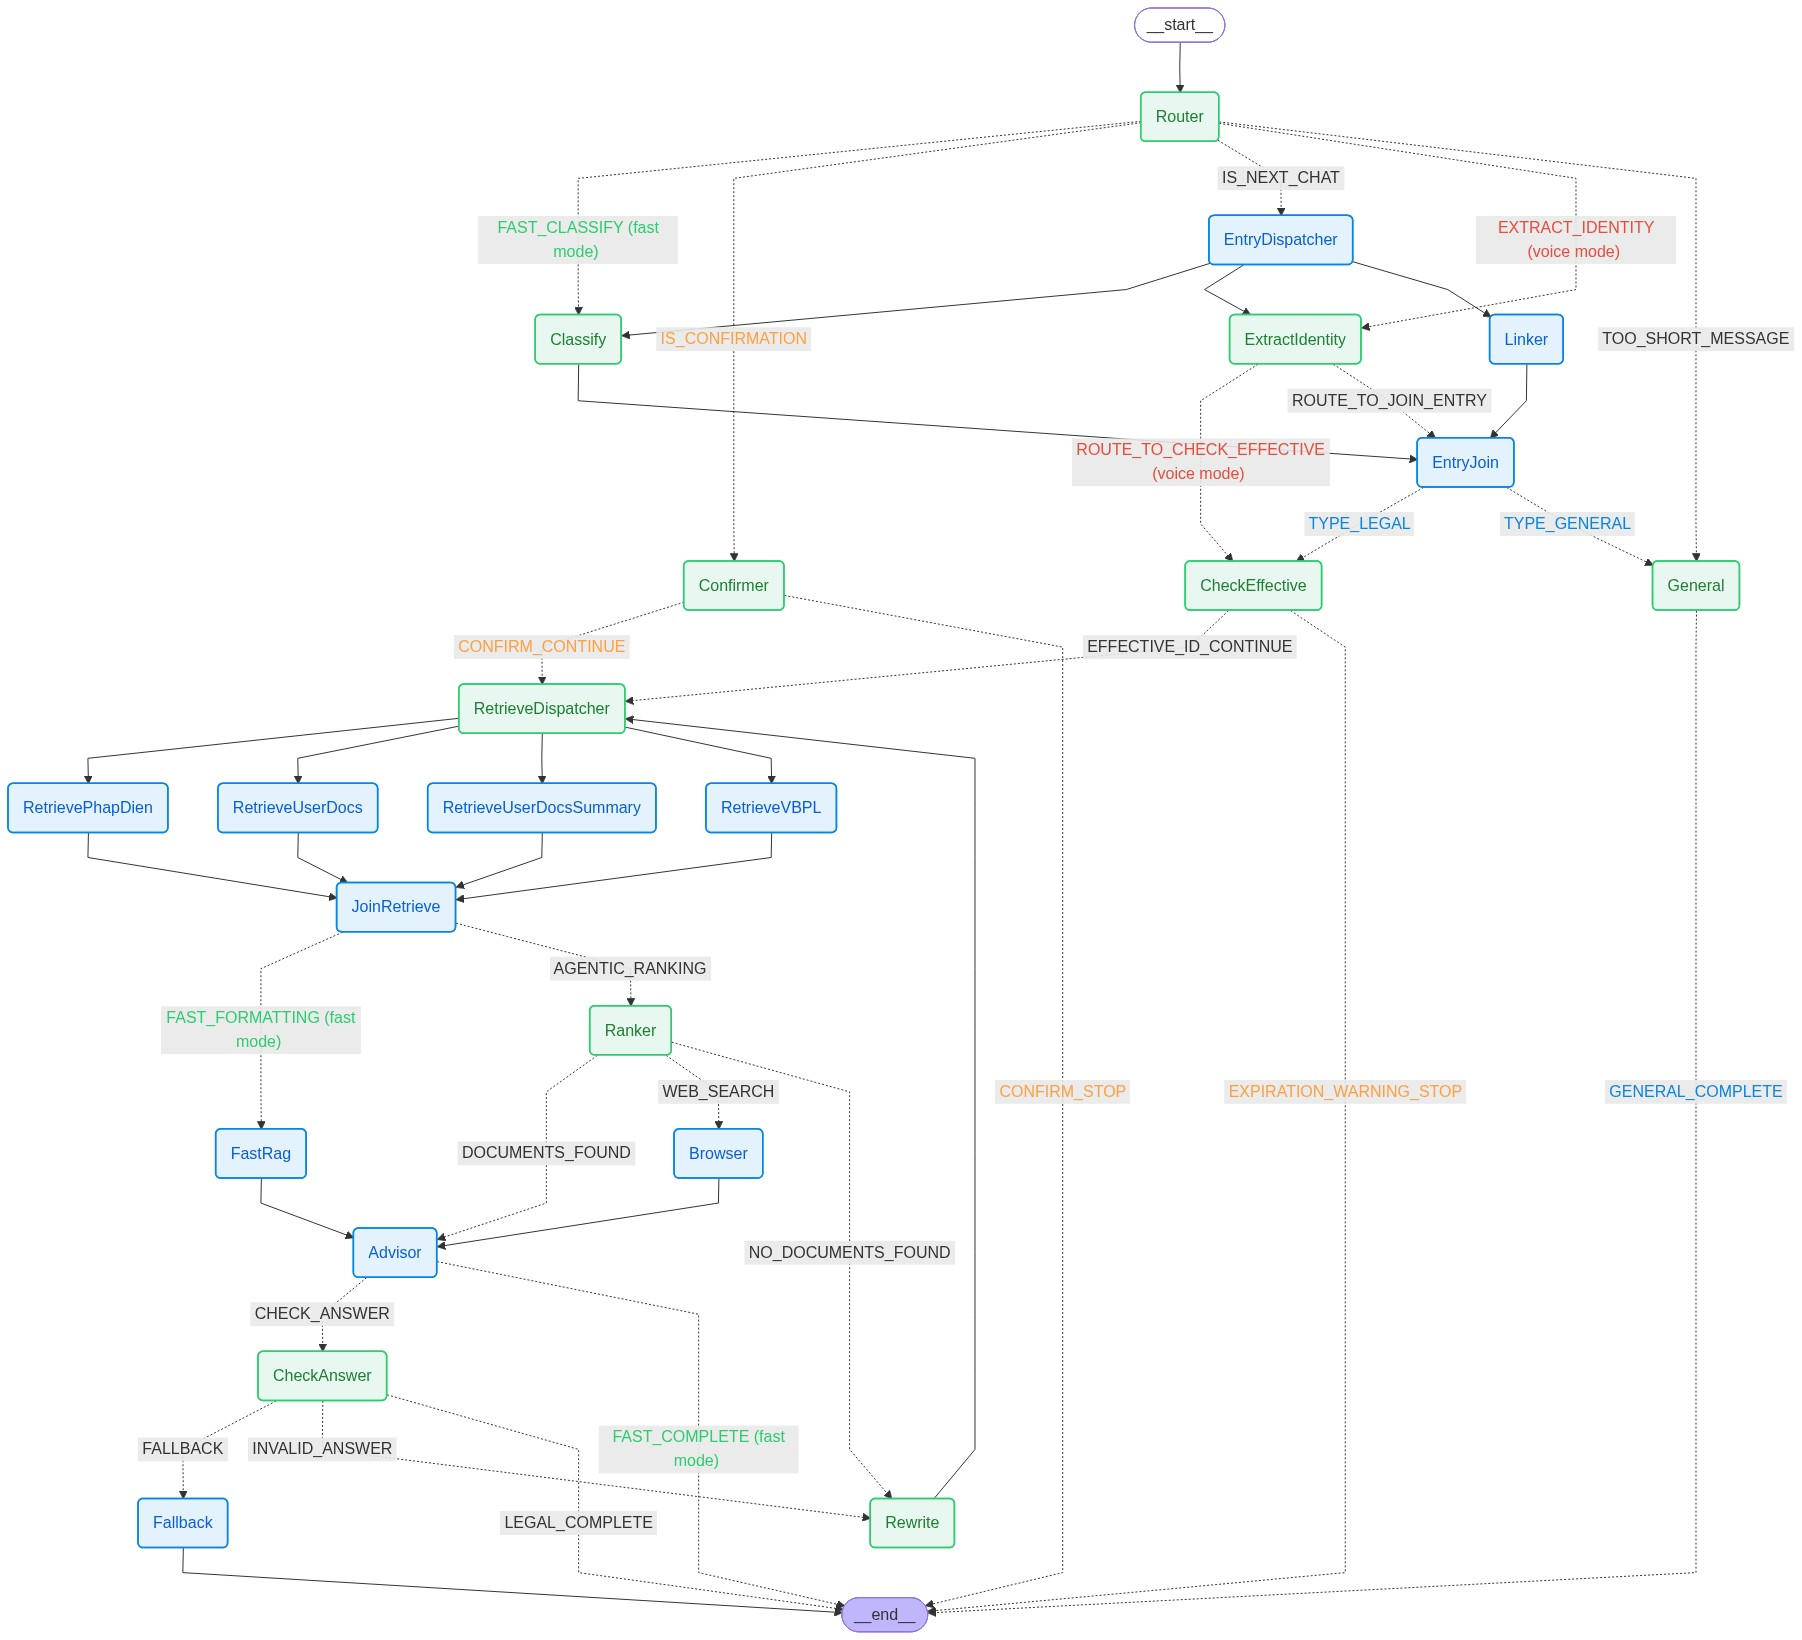
\includegraphics[width=\linewidth,height=0.74\textheight,keepaspectratio]{pictures/LangGraph/LangGraph0.png}
\caption{Sơ đồ LangGraph của hệ thống}
\end{figure}

\note{

Đây là toàn bộ sơ đồ Agentic RAG của hệ thống

\hrule

Ở chế độ fast RAG

chỉ dùng phân loại

để giảm tài nguyên truy xuất dữ liệu

và thực hiện trả lời

với dữ liệu đã truy xuất

\hrule

phù hợp với kiến trúc RAG cơ bản

\hrule

Ở chế độ voice

do đã có LLM ở sử dụng tool calling

VÀ

Người dùng không nhập đường dẫn bằng giọng nói

nên sẽ bỏ qua phân loại và xử lý đường dẫn

\hrule

thực hiện luôn việc trích xuất số hiệu VBPL

}
\end{frame}

% đây là toàn bộ sơ đồ ây gen tíc rag của hệ thống

% ở chế độ fast rag chỉ dùng phân loại để giảm tài nguyên truy xuất dữ liệu

% và thực hiện trả lời với dữ liệu đã truy xuất phù hợp với kiến trúc rag cơ bản

% ở chế độ voice do đã có llm ở sử dụng tool côn linh

% và người dùng không nhập đường dẫn bằng giọng nói

% nên sẽ bỏ qua phân loại và xử lý đường dẫn

% thực hiện luôn việc trích xuất số hiệu văn bản pháp luật
